
\section{Problems of classical I2A}
\begin{frame}{Problems of classical I2A}
    \begin{PraesentationAufzaehlung}
        \item not scalable to large states - rollouts are slow
        \item not scalable to large action spaces - one rollout per action
        \item environment model has problems predicting far into the future
    \end{PraesentationAufzaehlung}
\end{frame}

\begin{frame}
	\frametitle{Classical I2A rollout}
	\begin{figure}[h]
		\centering
		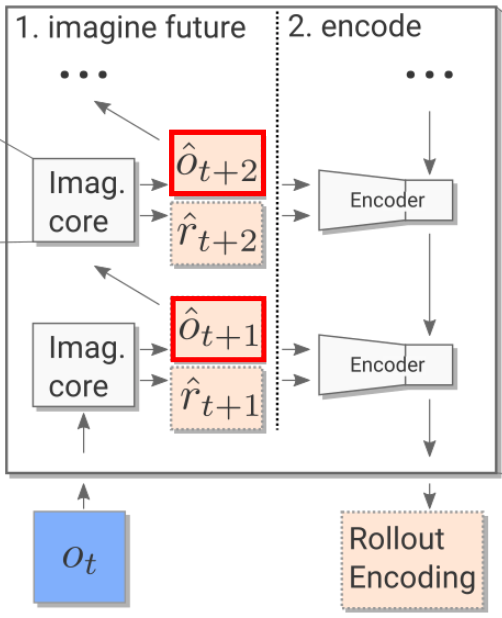
\includegraphics[height=0.7\textheight]{./latent_i2a_images/SingleImaginationRollout_marked.png}
	\end{figure}
\end{frame}

\begin{frame}{Solution to large states}
	\begin{PraesentationAufzaehlung}
	    \item compress state into a latent representation
	    \item compute rollout in latent space
	\end{PraesentationAufzaehlung}
\end{frame}


%reference to 2nd paper
\begin{frame}
    \PraesentationUeberschriftZweizeilig{
Learning and Querying Fast Generative Models for Reinforcement Learning}{Buesing et al.(2018)}

\begin{PraesentationAufzaehlung}
    \item 
    \item 
    \item 
\end{PraesentationAufzaehlung}

\end{frame}
\clearpage



%Introduction of Latent Environment Model types
\begin{frame}
	\frametitle{Environment Model Architectures}
	\begin{multicols}{3}
	dSSM-DET\\
	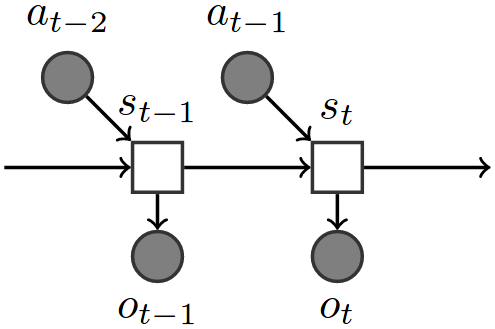
\includegraphics[width=\columnwidth]{./latent_i2a_images/dSSM_DET_architecture.png}
	\columnbreak
	dSSM-VAE\\
	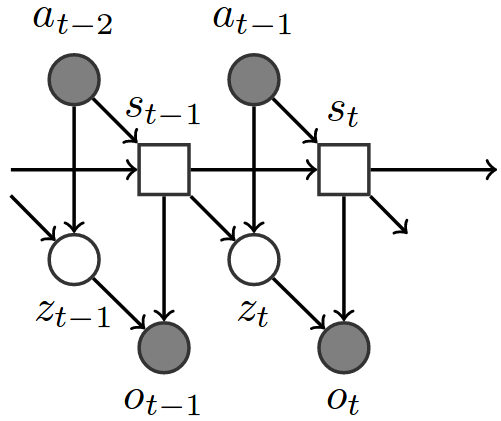
\includegraphics[width=\columnwidth]{./latent_i2a_images/dSSM_VAE_architecture.png}
	\columnbreak
	sSSM \\
	%\begin{figure}[H]
		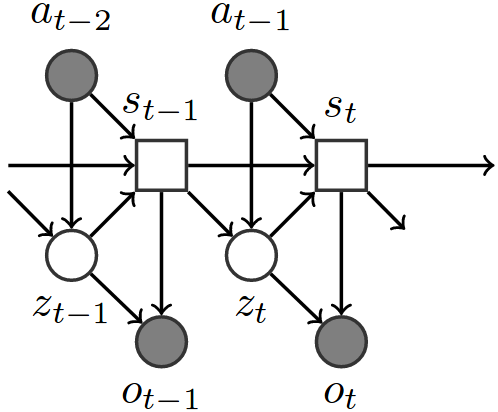
\includegraphics[width=\columnwidth]{./latent_i2a_images/sSSM_architecture.png}
	%\end{figure}
	\end{multicols}
\end{frame}

%dSSM-DET
\begin{frame}
	\frametitle{dSSM-DET}
	\begin{multicols}{2}
		\begin{figure}[h]
			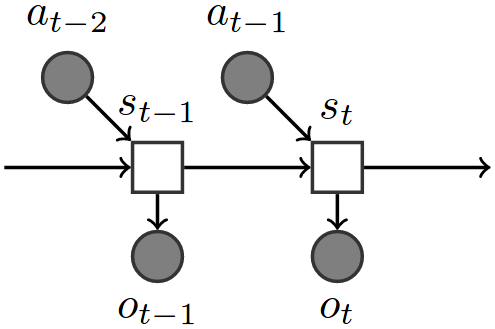
\includegraphics[width=0.4\textwidth]{./latent_i2a_images/dSSM_DET_architecture.png}	
		\end{figure}
		\columnbreak
		$s_t$: compact latent representation of state at time t\\
		$a_t$: action at time t\\
		$o_t$: predicted output
	\end{multicols}
\end{frame}

%dSSM-VAE
\begin{frame}
	\frametitle{dSSM-DET}
	\begin{multicols}{2}
		\begin{figure}[h]
			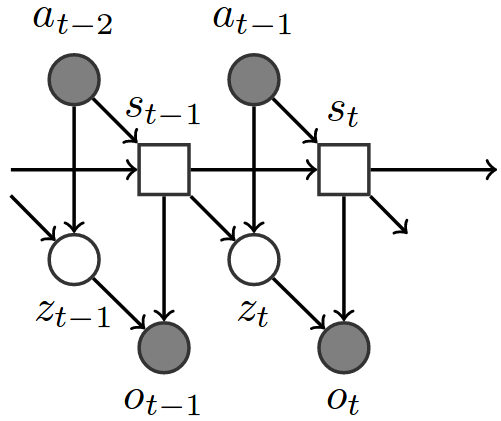
\includegraphics[width=0.4\textwidth]{./latent_i2a_images/dSSM_VAE_architecture.png}	
		\end{figure}
		\columnbreak
		$z_t$: latent variable sampled from gaussian distribution given by learnable mean and standard deviation
	\end{multicols}
\end{frame}


%closer examination of sSSM - dSSM types can be seen as subtypes of sSSM
\begin{frame}
	\frametitle{sSSM}
	dSSM variants can be seen as simplifications of sSSM \\
	\begin{multicols}{2}
		\begin{figure}[h]
			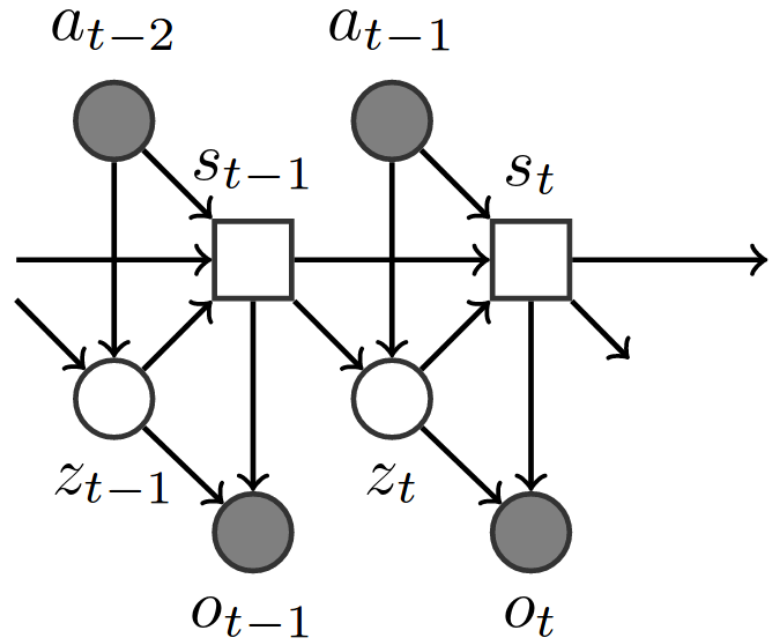
\includegraphics[width=0.4\textwidth]{./latent_i2a_images/sSSM2.png}	
		\end{figure}
		\columnbreak
	\end{multicols}
\end{frame}


\begin{frame}
	\frametitle{Environment Model Decoder}
	\begin{multicols}{2}
		\begin{figure}[h]
			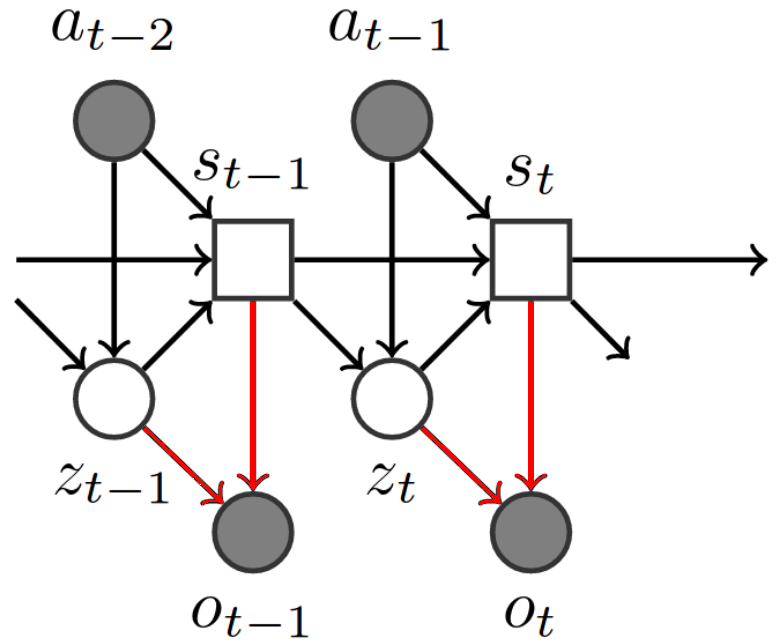
\includegraphics[width=0.4\textwidth]{./latent_i2a_images/sSSM2_decoder_marked.png}	
		\end{figure}
		\columnbreak
		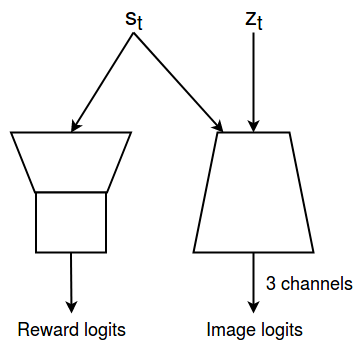
\includegraphics[width=0.4\textwidth]{./latent_i2a_images/LatentSpaceDecoder.png}
	\end{multicols}
\end{frame}

\begin{frame}
	\frametitle{Environment Model State Transition}
	\begin{multicols}{2}
		\begin{figure}[h]
			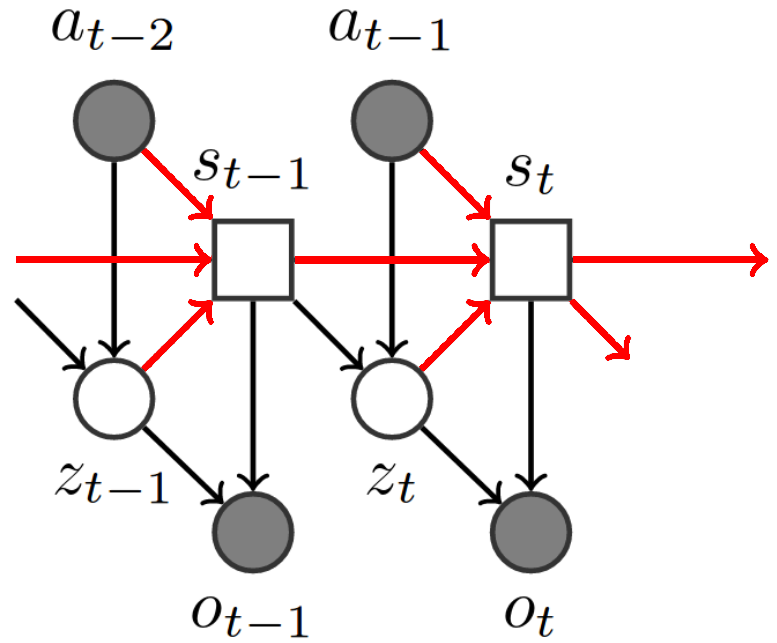
\includegraphics[width=0.4\textwidth]{./latent_i2a_images/sSSM2_state_transition_marked.png}	
		\end{figure}
		\columnbreak
		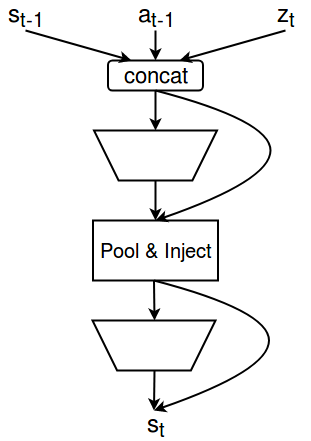
\includegraphics[width=0.4\textwidth]{./latent_i2a_images/LatentSpaceTransition.png}
	\end{multicols}
\end{frame}


\begin{frame}{Training the Environment Model}
    dSSM-DET
    Maximum Likelihood Estimation:
    \begin{equation}
            L(\theta) = \log p_{\theta}(o_{1:T}|a_{0:T-1}, \hat{o}_0)
        \end{equation}
        $\hat{o}_0$: initial context\\
        the encodings of the last 3 observations are used to generate $s_0$ in a learnable way
    
\end{frame}

\begin{frame}{Training the Environment Model}
    sSSM
        Evidence Lower Bound:
        \begin{equation}
        \begin{aligned}
            ELBO_q(\theta) = \sum_{t=1}^T \EX_q[\log p(o_t|s_t) + \log p(z_t|s_{t-1}, a_{t-1})\\ - \log q(z_t|s{t-1}, a_{t-1}, o_t)]
        \end{aligned}
        \end{equation}
        
        ELBO = reconstruction loss + KL-Div between true and approximated posterior\\
        $p(o_t|s_t)$: Bernoulli Distribution
        --> Reconstruction loss: equal to binary cross entropy
        TODO: warum bernoulli - image channels interpreted as probability distribution
        TODO: image
        
        TODO: how does the reward loss work
        TODO: maximizing ELBO is minimizing KL-Div is maximizing likelihood
\end{frame}

\begin{frame}

\end{frame}


\begin{frame}
	\frametitle{Comparison of Environment Model architectures}
	\begin{PraesentationAufzaehlung}
		\item stochastic architectures perform better at predicting the future\\
		\item I2A seems to have difficulties learning from the output of sSSM
		\item dSSM-DET performs best when combining it with I2A
	\end{PraesentationAufzaehlung}
\end{frame}




\begin{frame}{dSSM-DET rollout prediction}
    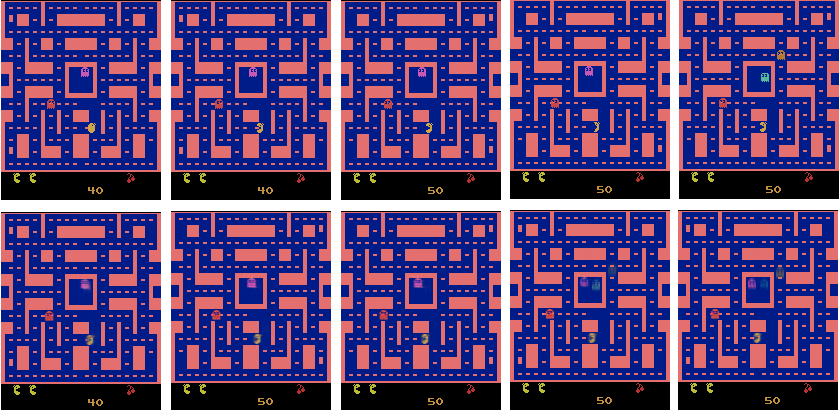
\includegraphics[width=\textwidth]{./latent_i2a_images/dSSM_rollout_prediction.png}
\end{frame}

%TODO video


\begin{frame}
	\frametitle{Why is MsPacman a hard prediction problem?}
	\begin{PraesentationAufzaehlung}
		\item state size: 160x200x3
		\item sprites of pacman and ghosts are not static
		\item blinking objects, essential objects are not seen in all frames
		\item ghosts follow certain rules - the environment model has to learn them to predict ghost behaviour
		\item some reward-types are very sparse
	\end{PraesentationAufzaehlung}
\end{frame}

    
\begin{frame}{Environment Model training loss}
   \begin{figure}
       \centering
        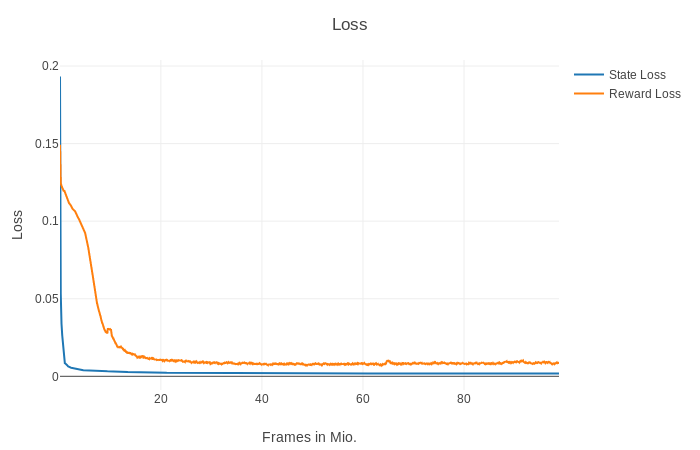
\includegraphics[width=\textwidth]{./latent_i2a_images/EnvironmentModel_dSSM-DET_training.png}
    \end{figure}
\end{frame}




\begin{frame}
TODO: changes to I2A architecture when using latent space
\end{frame}

\begin{frame}{dSSM-DET MsPacman - TODO: placeholder?}
    \begin{figure}
        \centering
        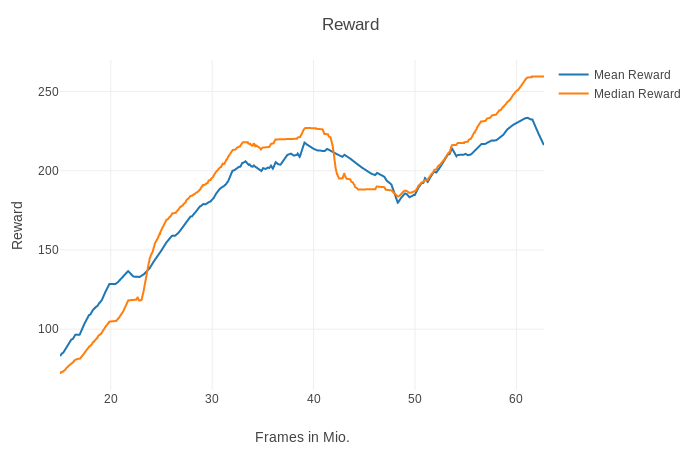
\includegraphics[width=\textwidth]{./latent_i2a_images/dSSM_DET_MsPacman.png}
    \end{figure}
\end{frame}


\begin{frame}
	\frametitle{Results}
	\begin{PraesentationAufzaehlung}
		\item pytorch framework for I2A
		\item implementation of latent environment model generation
		\item implementation of I2A using the latent space approach
	\end{PraesentationAufzaehlung}
	
	\bigskip
	Our code will be published on github.\\
	If you are interested send us an email to get the link.
\end{frame}


%Future Work
\begin{frame}
	\frametitle{Potential future work}
	\begin{PraesentationAufzaehlung}
		\item use the compact latent representation for both paths
	\item use GANs for the environment model
	\item try impact of smaller latent space, the latent space in the paper is still pretty large
	
	\item continue to train environment model together with the policy network\\
	For comlplex problems other state-of-the-art methods may not be good enough to get a representative training set for the environment model training.
	\item select promising actions to focus rollouts on
	\end{PraesentationAufzaehlung}
\end{frame}

